\documentclass[sigconf, nonacm]{acmart}

%% \BibTeX command to typeset BibTeX logo in the docs
\AtBeginDocument{%
  \providecommand\BibTeX{{%
    \normalfont B\kern-0.5em{\scshape i\kern-0.25em b}\kern-0.8em\TeX}}}

%% Rights management information.  This information is sent to you
%% when you complete the rights form.  These commands have SAMPLE
%% values in them; it is your responsibility as an author to replace
%% the commands and values with those provided to you when you
%% complete the rights form.
\setcopyright{acmcopyright}
\copyrightyear{2018}
\acmYear{2018}
\acmDOI{XXXXXXX.XXXXXXX}

%% These commands are for a PROCEEDINGS abstract or paper.
\acmConference[Conference acronym 'XX]{Make sure to enter the correct
  conference title from your rights confirmation emai}{June 03--05,
  2018}{Woodstock, NY}
%
%  Uncomment \acmBooktitle if th title of the proceedings is different
%  from ``Proceedings of ...''!
%
%\acmBooktitle{Woodstock '18: ACM Symposium on Neural Gaze Detection,
%  June 03--05, 2018, Woodstock, NY} 
\acmPrice{15.00}
\acmISBN{978-1-4503-XXXX-X/18/06}

% TikZ and plotting tools
\usepackage{tikz, pgfplots}
\usepackage{subcaption}
\pgfplotsset{compat=1.18}
\usetikzlibrary{positioning}

% Layer colors
\def\ConvColor{rgb:yellow,5;red,2.5;white,5}
\def\ConvReluColor{rgb:yellow,5;red,5;white,5}
\def\PoolColor{rgb:red,1;black,0.3}
\def\DcnvColor{rgb:blue,5;green,2.5;white,5}
\def\SoftmaxColor{rgb:magenta,5;black,7}

% Miscellany
\usepackage{import}
\usepackage{multirow}
\usepackage{svg}
\usepackage{import}
\subimport{layers/}{init}
\newcommand{\ra}[1]{\renewcommand{\arraystretch}{#1}}


%%
%% end of the preamble, start of the body of the document source.
\begin{document}

%%
%% The "title" command has an optional parameter,
%% allowing the author to define a "short title" to be used in page headers.
\title{Wrangling with the paper ``Unsupervised Space Partitioning for Nearest Neibhour Search''}

%%
%% The "author" command and its associated commands are used to define
%% the authors and their affiliations.
%% Of note is the shared affiliation of the first two authors, and the
%% "authornote" and "authornotemark" commands
%% used to denote shared contribution to the research.
\author{Michael Darmanis}
\authornote{Both authors contributed equally to this project.}
\email{mdarm@di.uoa.gr}
\author{Stathis Kotsis}
\authornotemark[1]
\email{efstathkot@di.uoa.gr}
\affiliation{%
  \institution{National and Kapodistrian University of Athens}
  \city{M149 - Database Systems}
  \country{Spring 2023}
}


%%
%% By default, the full list of authors will be used in the page
%% headers. Often, this list is too long, and will overlap
%% other information printed in the page headers. This command allows
%% the author to define a more concise list
%% of authors' names for this purpose.
\renewcommand{\shortauthors}{Darmanis and Kotsis}

%%
%% The abstract is a short summary of the work to be presented in the
%% article.
\begin{abstract}
    This report presents a series of extensions to the paper "Unsupervised Space Partitioning for Approximate Nearest Neighbour Search". The original focus of the paper is to develop an efficient approach for approximate nearest neighbour search in high-dimensional spaces, which is a critical problem in various domains such as image retrieval, recommendation systems, and natural language processing. The improvements described in this report aim at further optimising the efficiency and accuracy of the approach. First, Principal Component Analysis (PCA) is introduced as a preprocessing step to reduce the dimensionality of the feature space and retain the most informative components. Second, the Mahalanobis distance metric is used to account for correlations between variables, making it more suitable for high-dimensional data than the traditional Euclidean distance. Third, a convolutional neural network is implemented as an additional model for the ensembling mechanism and integrated into the existing structure. Fourth, the ensembling process is modified to incorporate different model types, including linear models, neural networks and convolutional neural networks (CNNs), while adding seamless integration for any type of potential future model, allowing for greater flexibility in model selection. Fifthly, product vector quantization will be implemented and added as an option for more fine-grained unsupervised neighbour search on top of the existing model. Finally, an attempt to integrate the Hierarchical Navigable Small Worlds (HNSW) algorithm is documented, although this extension is only partially implemented due to time constraints. The report provides the rationale, mathematical formulations, and initial Python code for each enhancement. It also provides space to document experimental results comparing the original and improved settings. Through these improvements, the report contributes to the ongoing effort to optimise approximate nearest neighbour search.
\end{abstract}

%%
%% The code below is generated by the tool at http://dl.acm.org/ccs.cfm.
%% Please copy and paste the code instead of the example below.
%%
\begin{CCSXML}
<ccs2012>
 <concept>
  <concept_id>10010147.10010257.10010293.10010294</concept_id>
  <concept_desc>Computing methodologies~Neural networks</concept_desc>
  <concept_significance>500</concept_significance>
 </concept>
 <concept>
  <concept_id>10010147.10010257.10010293.10010296</concept_id>
  <concept_desc>Computing methodologies~Learning paradigms</concept_desc>
  <concept_significance>300</concept_significance>
 </concept>
 <concept>
  <concept_id>10002950.10003714.10003716</concept_id>
  <concept_desc>Mathematics of computing~Mathematical software performance</concept_desc>
  <concept_significance>300</concept_significance>
 </concept>
 <concept>
  <concept_id>10010147.10010371.10010382.10010383</concept_id>
  <concept_desc>Computing methodologies~Image processing algorithms</concept_desc>
  <concept_significance>200</concept_significance>
 </concept>
 <concept>
  <concept_id>10002950.10003712.10003716.10011138.10010043</concept_id>
  <concept_desc>Mathematics of computing~Approximation algorithms</concept_desc>
  <concept_significance>200</concept_significance>
 </concept>
</ccs2012>
\end{CCSXML}

\ccsdesc[500]{Computing methodologies~Neural networks}
\ccsdesc[300]{Computing methodologies~Learning paradigms}
\ccsdesc[300]{Mathematics of computing~Mathematical software performance}
\ccsdesc[200]{Computing methodologies~Image processing algorithms}
\ccsdesc[200]{Mathematics of computing~Approximation algorithms}

%%
%% Keywords. The author(s) should pick words that accurately describe
%% the work being presented. Separate the keywords with commas -- I do not like commas though :)
\keywords{approximate nearest neighbor search; unsupervised space partitioning; principal component analysis; mahalanobis distance; ensemble models; convolutional neural networks; hierarchical navigable small worlds; high-dimensional data}

%% A "teaser" image appears between the author and affiliation
%% information and the body of the document, and typically spans the
%% page.

\received{25 June 2023}

%%
%% This command processes the author and affiliation and title
%% information and builds the first part of the formatted document.
\maketitle

\section{Introduction}
This report summarises the improvements made to the paper entitled ``Unsupervised Space Partitioning for Approximate Nearest Neighbour Search''. The aim of these improvements was to increase the performance and capabilities of the proposed approach. The improvements include the use of PCA as a pre-processing stage, the adoption of the Mahalanobis distance metric, and modifications to the ensembling process to allow for the incorporation of linear, neural, and CNN models. In addition, the report documents an attempt at improvement involving partial implementation of the Hierarchical Navigable Small Worlds (HNSW) approach. The report will outline the rationale behind each improvement and provide a space to record the results of experiments conducted based on the original settings.

\section{Implemented Improvements}

\subsection{Principal Component Analysis (PCA) Preprocessing}
Principal Component Analysis (PCA) \cite{pca-origin} was used as a preprocessing step to reduce the dimensionality of the feature space. By retaining the principal components that explain the most variance in the data, it is possible to reduce computational complexity without losing critical information. This reduction in dimensionality is particularly beneficial for high-dimensional datasets such as images, where each pixel is considered a feature. PCA can help filter out noise and irrelevant features, leading to better generalisation and faster training times.

The mathematical formulation of PCA is as follows

\begin{equation}
Y = X \times W
\end{equation}

where $Y$ is the matrix of principal components, $X$ is the original data matrix, and $W$ is the matrix of loadings or weights.

For datasets such as MNIST and SIFT, which contain high-dimensional data points representing images, the use of PCA as a preprocessing step is expected to be advantageous. In MNIST, each image is 28x28 pixels, resulting in 784 dimensions, and in SIFT, each image is represented by a 128-dimensional feature vector. PCA can significantly reduce the number of dimensions while retaining the features essential for classification or nearest neighbour search.

In addition, PCA can sometimes improve the performance of certain algorithms by removing correlations between features, which can be beneficial for algorithms that assume feature independence.

It's important to note that the choice of the number of principal components to retain is a critical decision. In our implementation, we decided to keep the components that retained 95\% of the original variance.

\subsection{Mahalanobis Distance Metric}
The Mahalanobis distance metric was introduced as an alternative to the Euclidean distance commonly used in various machine learning algorithms. The Mahalanobis distance takes into account correlations between variables and variance along different dimensions, making it more appropriate for high-dimensional data where features may not be independent.

The Mahalanobis distance between two points $x$ and $y$ is defined as

\begin{equation}
D_M(x, y) = \sqrt{(x-y)^T \times S^{-1} \times (x-y)}
\end{equation}

where $S$ is the covariance matrix of the data.

Unlike the Euclidean distance, which treats each dimension equally, the Mahalanobis distance takes into account the dispersion and correlation of data in different dimensions. This can be particularly useful in scenarios where the size and distribution of features vary, as it standardises the data based on their distribution.

For datasets such as MNIST and SIFT, where the features represent pixel intensities or local image descriptors, the distribution and correlations of the features are important aspects to consider. The Mahalanobis distance can capture the intrinsic geometry of such datasets more accurately compared to the Euclidean distance.

Furthermore, although more computationally intensive, the Mahalanobis distance is scale-invariant and correlates well with human perception of similarity. It's particularly effective in applications such as image recognition, anomaly detection and clustering, where understanding the underlying geometry of the data is critical.

\subsection{Ensembling Process with Different Model Types}
Ensembling is a broad category of machine learning techniques that combine multiple models to make predictions. Those models are called base learners. If all the models in the ensemble are of the same type then they are called homogeneous ensembles while they are called heterogeneous learners if different learning algorithms are used. The three main categories of Ensembling are bagging, stacking and boosting.Bagging mainly involves feeding different samples of a dataset into base learners in parallel and taking usually the average of the predictions as the output of the model.The average of the predictions is only one possible method to obtain the final results. Weighted averaging and voting are also viable options. With Stacking, various different base learners fit on the same data samples and the output of the base learners is fed into a Meta Learning Model with the initial dataset labels as the targets. The meta learner decides how to combine the models' predictions.Finally boosting\cite{boosting} is based on sequential models. In particular each base learner makes predictions on the same data and each subsequent model tries to correct the mistakes of previous models by assigning bigger weights to the datapoints wrongly predicted. The final output is a weighted average of the predictions from each model according to it's predictive power. In essence, boosting tries to convert weak learners, which perform slightly better than random guessing to strong learners, models with high accuracy\cite{ensembling}. 

In the original work the ensemble model is based on  Boosted Search Forest\cite{bforest} which uses AdaBoost\cite{adaboost} for the correction of wrong partitions predictions in a sequential manner. Each model focuses on the points which were wrongly partitioned in the previous model and tries to improve those predictions based on a loss function.

The ensemble process has been modified to allow different types of models to be included. This change allows greater flexibility in the type of models that can be included in the ensemble. In particular, instead of training tree nodes of the same model type, the implementation has been extended to support the construction and training of linear regression models, convolutional and neural networks. By combining these different types of models, the ensemble can potentially achieve higher performance than any single model alone. This is particularly useful for datasets such as MNIST, which contains images of handwritten digits, and SIFT, which contains local image descriptors. CNNs can be effective at capturing spatial patterns in images, while linear models and neural networks can capture other types of relationships in the data: for example, CNNs can learn to recognise the strokes in handwritten digits, while a neural network can capture how these strokes combine to form different numbers. Linear models can provide a baseline that's less prone to overfitting. Linear models are relatively simple and interpretable, but may not capture complex patterns in the data. Neural networks are more flexible and can model non-linear relationships, but are prone to overfitting on small data sets. Convolutional Neural Networks (CNNs) are particularly effective for image data as they can automatically learn to recognise patterns in the spatial structure of the data. 

The process of ensemble training with different models can be seen in Figure~\ref{fig:ensemble}. The first base learner, a Neural Network here, is fed the points in the dataset and does some predictions, then the datapoints are weighted and the mispredicted are assigned higher weights. After that they are fed to a cnn model which corrects some mistakes from the previous model. Following the same process, the final model is then able to classify all the partitions correctly.

Furthermore, we argue that the support of different models could be used to design a Stacking Ensembling method, as an alternative to Boosting, where the final predictions and the task of optimally combining the models is done by a Meta Learner, when the complexity of the dataset is high and simple averaging schemes do not produce the desired results. We'll leave the design of such a model and its integration to future work.

\begin{figure}[ht]
\centering
  \includegraphics[width=0.45\textwidth]{plots/ensembling.jpg}
  \caption{ This figure is a simplification of the main scheme used for training the base learners for our task, which is similar to a classification task.} 
  \label{fig:ensemble}
\end{figure}



\subsection{CNN Implementation and Integration}

The ensemble was extended to include Convolutional Neural Networks (CNNs), which are particularly adept at handling image data by efficiently capturing spatial structures\cite{cnn}. This inclusion could potentially be beneficial for the MNIST dataset, with its grey-scale images of handwritten digits, as CNNs excel at recognising intricate spatial patterns such as strokes and lines. Similarly, for the SIFT dataset, which deals with feature descriptors for image matching, CNNs are able to identify key features in images. In particular, the CNN model is designed to work for the MNIST dataset and it's variants (Fashion-MNIST), but extension to other datasets is trivial and can be easily achieved with just a few changes to the implementation, provided that the feature dimensions can be reshaped into a square matrix. The convolutional neural network architecture used consists of three convolutional layers and two linear layers.The input to the convolutional neural network is a tensor of shape (batch size,1,28,28), which is a batch of the square image matrices of the MNIST dataset. The first convolutional layer applies a convolution with 6 kernels, kernel size 3x3 and stride 1. This is followed by ReLu activation, a max-pooling layer with kernel size 2x2 and stride 2, and a batch normalisation layer. The second convolutional layer uses 16 kernels of size 3x3 and stride 1, followed by ReLu activation and max pooling of kernel size 2x2. The final convolutional layer uses 120 kernels of size 3x3 followed by ReLu. The output is then flattened and fed into a linear layer with ReLu activation. This produces a vector of size n\_hidden for each batch, where n\_hidden is specified by the user. The default value is 84.

You can see a rough sketch of the CNN architecture, at Figure~\ref{cnn} of Appendix~\ref{sec:appendix}, and the number of layers and parameters in each layer.

% make cnn
\subsection{Ensembling with Product Vector Quantization Pipeline}

Since the main task of the unsupervised partitioning model is to divide the space into multiple partitions, each of which is likely to contain potential neighbours, the task of retrieving the top-k neighbours of query points from the generated bins can alternatively be performed using a simple product quantization\footnote{Our implementation of the code was heavily influenced by this tutorial: \url{https://github.com/jankrepl/mildlyoverfitted}}. Product quantization \cite{pquantize} is the process of compressing data into a smaller space. This is achieved by encoding each data vector into a smaller encoding, a symbolic representation. This method drastically reduces the memory consumption of the data vectors.

In order to better fine-tune the top-k neighbours, we can therefore use a two-step pipeline where

(1)The Unsupervised Space partitioning method first divides the space into multiple partitions, reducing the search space for finding the top-k neighbours.


(2)The points in each produced bin are encoded and inserted into an index using a quantization process. After the index is created the top-k neighbours for each point in the bin can be retrieved.

The quantization process is as follows : The points in each partition are split into subvectors and for each subvector a number of cluster centroids are produced. The number of centroids and the dimensions of the subvectors can be easily parametrized by the user. Then the distances of the centroids for each subvector are calculated and stored since they will be used as an index later. The centroids are then fit using a clustering Algorithm like K-means and each subvector is assigned to it's closest centroid, thus building a codebook which includes all the data points' unique encodings. These are the unique symbolic representations of all the data points. Since we now have the symbolic representation of the datapoints and the distances of the centroids, finding the top-k neighbours for each data point is easy.The query point's subvectors distances with all the other points' subvectors in the codebook are retrieved using a lookup operation in the stored distances' tables and added together to form the total distance of the query point with any other point. The top-k smallest distances define the top-k nearest neighbours. Since the encoding of each data point is very small in comparison to the initial data point's dimensions, this method is characterized by very low memory usage and is great when low memory availability is expected. Testing the method on our dataset it seems that the real bottleneck is the number of cluster centroids and the number of samples in each bin since they must be compared with each other to store the distances. In our case 1000 query points from the test dataset were fed into the quantization process after the space partitioning took place and the top-10 neighbours were queried. The results for candidate set sizes of 3000-4000 points show that the method can be used as an additional step, to index the points of each returned bin and find  the nearest neighbours of each one of them after the distances have been calculated and stored but optimization steps are required in order to tackle the bottlenecks. Such optimization methods are available\cite{opmethods} but they are out of the scope of this work. The time required for finding the top-10 nearest neighbours for varying number of queries and quantization parameters using the simple quantization approach are presented in \ref{table:params} .


\begin{figure}[ht]
    \centering
    \includegraphics[width=0.45\textwidth]{plots/product_quantization_shape.jpg}
    \caption{Overview of the 2 step pipeline feeding the results of the Ensemble to the quantization process and then querying for the nearest neighbours.} 
  \label{fig:quantization}
\end{figure}


\begin{table}[ht]
\centering
\caption{Query time for finding the top-10 nearest neighbours for varying number of query points, of dimensions 784, 4 centroids per subvector and 16 subvectors, in an average candidate size of 3000}
\begin{tabular}{c c}
\toprule
\texttt{\#} Query points & Time (m)\\ 
\midrule
100 &  1.85\\ 
500 & 5.92\\ 
1000 & 15.7\\
\bottomrule
\end{tabular}
\label{table:params}
\end{table}


\section{Experimental Setup \& Results}

In this section, we present the experimental setup and results obtained from various modifications made to the baseline model presented in the original paper. The experiments had the same settings as the original paper, using the same datasets and evaluation metrics and protocols\cite{neural}. Below, we enumerate the different modifications:

\begin{enumerate}
    \item \textbf{Baseline Model:} As a reference, we first established a baseline by using the original models presented in the paper, which includes Neural Networks and Logistic Regression.
    
    \item \textbf{Principal Component Analysis (PCA) Preprocessing:} We applied PCA as a preprocessing step to reduce the dimensionality of the feature space. This experiment aimed to understand the effect of dimensionality reduction on the model's performance.
    
    \item \textbf{Multimodel Ensembling:} We modified the ensembling process to incorporate different model types, including linear models and neural networks (not convolutional neural networks). This aimed to observe the effects of using a diverse set of models in the ensemble on the performance metrics.
    
    \item \textbf{Mahalanobis Distance Metric:} We adopted the Mahalanobis distance metric as an alternative to the Euclidean distance. This experiment aimed to understand the impact of accounting for correlations between variables in high-dimensional data on the model's performance.
    
    \item \textbf{Convolutional Neural Networks (CNNs):} In this experiment, we introduced Convolutional Neural Networks (CNNs) for feature extraction from raw data. The experiment involved the creation of a CNN architecture with several convolutional and pooling layers, followed by fully connected layers. The objective was to explore the efficacy of CNNs in capturing spatial patterns in the data and evaluate their performance compared to traditional Neural Networks. It's important to note that we did not apply CNNs on SIFT features because padding was required, and we had time limitations.
\end{enumerate}

\subsection{Results and Discussion}

\subsubsection{RNN-recall}

In terms of quality and accuracy of partitioning, it's interesting that PCA outperformed the original method for the 16-bin partition, especially given the relatively small feature space (see Figure~\ref{sift-16}). However, the performance of PCA for MNIST was poor. This could be due to PCA's tendency to capture global structures, which may not be as effective when dealing with high-dimensional data such as MNIST. On the contrary, for the 256 partition scheme (see Figures~\ref{sift-256} and \ref{mnist-256}), all implementations showed a degradation in performance. In particular, Mahalanobis distance generated a single large bin containing almost the entire dataset, as shown in Figures 3 and 4. This could be because the Mahalanobis distance takes into account the covariance of the data and may not be able to distinguish individual clusters in high-dimensional space, leading to ineffective partitioning. The results suggest that the modifications are not generalisable and are not recommended for large space partitions.

The multi-model ensemble also performed as expected, although it had a similar accuracy to the original model in the SIFT dataset (see Figure~\ref{sift-16}).  One of the likely reasons for this is the inherent complexity and high dimensionality of the datasets. When different models with their own assumptions and biases are ensembled, the combined model may not necessarily account for the structure of the data effectively. In addition, ensembling can sometimes lead to increased computational overhead, which may have negated any performance gains.

One reason for this may be that the loss function does not effectively capture the complexity of high-dimensional data or the covariance structure. This is evident in the degradation of the results for the 256 partition scheme, where the implementations performed poorly in partitioning the space. A potential improvement could be to include additional terms in the loss function (see Appendix~\ref{sec:appendix}) that take into account the geometric and distributional properties of the data, or to explore alternative distance metrics and data representation techniques that are more appropriate for high-dimensional spaces.

\subsubsection{Average query execution time}

In terms of average query execution time, all methods showed faster response times for RNN-recall, especially with the 16-bin partition (see Table~\ref{tab:query-time}). This is expected for PCA as it reduces the dimensionality of the feature space, resulting in less computational overhead. Similarly, the Mahalanobis distance may be faster as it may effectively eliminate less important dimensions, thus reducing the computational time. The table shows that for MNIST with 1 bin, PCA and Mahalanobis had query times of 0.30 and 0.41, respectively, compared to 0.67 for the original method, an improvement of about 55\% and 39\%, respectively. For CNN, the query times were even lower at 0.23 for MNIST with 1 bin, which is an improvement of about 66\% compared to the original method. However, CNN was not applied to SIFT due to padding requirements and time constraints.

\begin{figure*}[h]
    \centering

    % Common legend for all subplots
    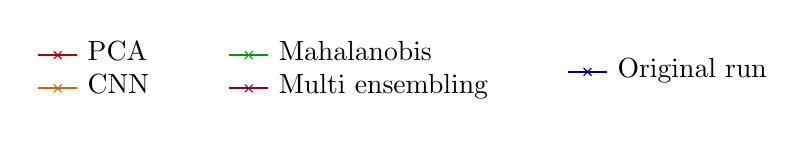
\begin{tikzpicture}[baseline=(current bounding box.center), remember picture]
        \node at (0,0) {};  % This is the new line
        \node[draw=none, anchor=north] at (current bounding box.north)
        {
            \begin{tabular}{@{}r@{ }l@{\hspace{1cm}}r@{ }l@{\hspace{1cm}}r@{ }l@{}}
                \raisebox{2pt}{\tikz{\draw[red!70!black, thick, solid] (0,0) -- ++(0.5,0);
                \draw[red!70!black, mark=x] plot coordinates {(0.25,0)};}} & PCA &
                \raisebox{2pt}{\tikz{\draw[green!60!black, thick, solid] (0,0) -- ++(0.5,0);
                \draw[green!60!black, mark=x] plot coordinates {(0.25,0)};}} & Mahalanobis & 
                \multirow{2}{*}{\raisebox{2pt}{\tikz{\draw[blue!50!black, thick, solid] (0,0) -- ++(0.5,0);
                \draw[blue!50!black, mark=x] plot coordinates {(0.25,0)};}}} & \multirow{2}{*}{Original run} \\
                \raisebox{2pt}{\tikz{\draw[orange!80!black, thick, solid] (0,0) -- ++(0.5,0);
                \draw[orange!80!black, mark=x] plot coordinates {(0.25,0)};}} & CNN &
                \raisebox{2pt}{\tikz{\draw[purple!70!black, thick, solid] (0,0) -- ++(0.5,0);
                \draw[purple!70!black, mark=x] plot coordinates {(0.25,0)};}} & Multi ensembling
            \end{tabular}
        };
    \end{tikzpicture}
    \vspace{10pt}
    
    \begin{subfigure}[b]{0.45\textwidth}
        \centering
        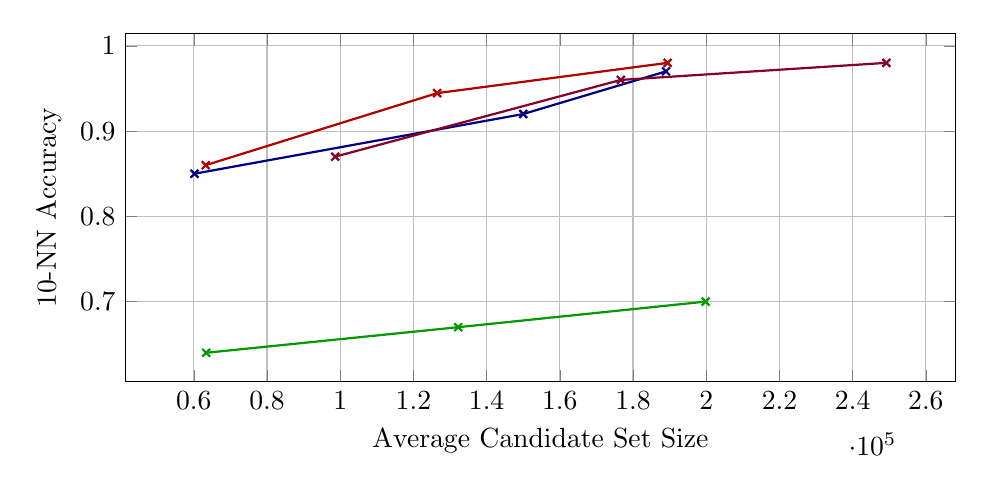
\begin{tikzpicture}
        \begin{axis}[
            width=\linewidth,
            height=6cm,
            grid=major,
            xlabel={Average Candidate Set Size},
            ylabel={10-NN Accuracy},
            mark options={solid}
        ]
        
        % Original
        \addplot[blue!50!black, thick, mark=x, mark size=2pt] coordinates {
            (60200, 0.85)
            (150000, 0.92)
            (189000, 0.97)
        };
        % PCA
        \addplot[red!70!black, thick, mark=x, mark size=2pt] coordinates {
            (63243, 0.86)
            (126475, 0.9445)
            (189444, 0.98)
        };
        % Mahalanobis
        \addplot[green!60!black, thick, mark=x, mark size=2pt] coordinates {
            (63386, 0.64)
            (132219, 0.67)
            (199818, 0.70)
        };
        % Multi-model ensembling 
        \addplot[purple!70!black, thick, mark=x, mark size=2pt] coordinates {
            (98631, 0.87)
            (176668, 0.96)
            (249204, 0.98)
        };
        \end{axis}
\end{tikzpicture} % Make sure the individual plot does not include a legend
        \caption{SIFT, 16 bins}
        \label{sift-16}
    \end{subfigure}
    \vspace{5mm}
    \hspace{5mm}
    \begin{subfigure}[b]{0.45\textwidth}
        \centering
        \input{plots/mnist-16} % Make sure the individual plot does not include a legend
        \caption{MNIST, 16 bins}
        \label{mnist-16}
    \end{subfigure}
    \hspace{5mm}
    \begin{subfigure}[b]{0.45\textwidth}
        \centering
        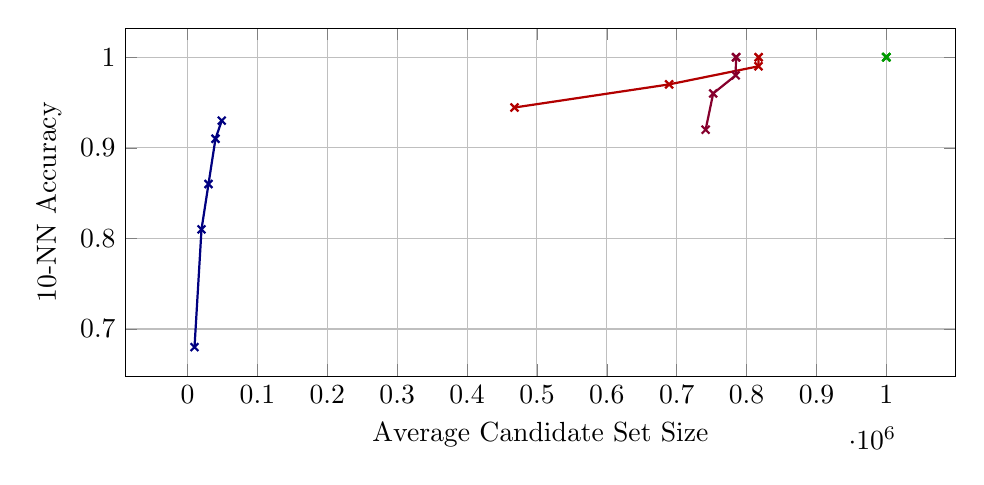
\begin{tikzpicture}
        \begin{axis}[
            width=\linewidth,
            height=6cm,
            grid=major,
            xlabel={Average Candidate Set Size},
            ylabel={10-NN Accuracy},
            mark options={solid}
        ]
        
        % Original
        \addplot[blue!50!black, thick, mark=x, mark size=2pt] coordinates {
            (10000, 0.68)
            (20000, 0.81)
            (30000, 0.86)
            (40000, 0.91)
            (49000, 0.93)
        };
        % PCA
        \addplot[red!70!black, thick, mark=x, mark size=2pt] coordinates {
            (467974, 0.9445)
            (689184, 0.97)
            (817024, 0.99)
            (817221, 1.0)
            (817221, 1.0)
        };
        % Mahalanobis
        \addplot[green!60!black, thick, mark=x, mark size=2pt] coordinates {
            (1000000, 1.0)
            (1000000, 1.0)
            (1000000, 1.0)
            (1000000, 1.0)
            (1000000, 1.0)
        };
        % Multi-model ensembling 
        \addplot[purple!70!black, thick, mark=x, mark size=2pt] coordinates {
            (741386, 0.92)
            (752203, 0.96)
            (784437, 0.98)
            (784865, 1.0)
            (785146, 1.0)
        };
        \end{axis}
\end{tikzpicture} % Make sure the individual plot does not include a legend
        \caption{SIFT, 256 bins}
        \label{sift-256}
    \end{subfigure}
    \hspace{5mm}
    \begin{subfigure}[b]{0.45\textwidth}
        \centering
        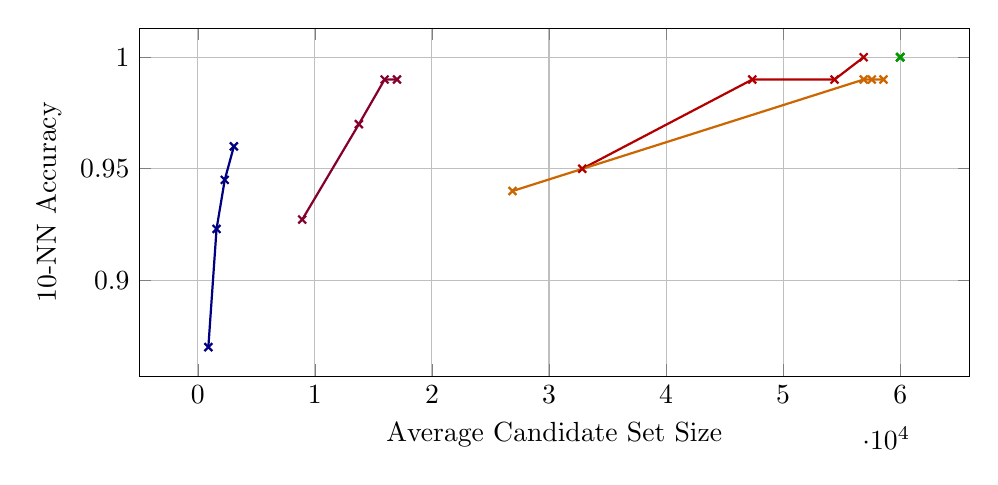
\begin{tikzpicture}
        \begin{axis}[
            width=\linewidth,
            height=6cm,
            grid=major,
            xlabel={Average Candidate Set Size},
            ylabel={10-NN Accuracy},
            mark options={solid}
        ]
        
        % Original
        \addplot[blue!50!black, thick, mark=x, mark size=2pt] coordinates {
            (900, 0.87)
            (1600, 0.923)
            (2300, 0.945)
            (3080, 0.96)
        };
        % PCA
        \addplot[red!70!black, thick, mark=x, mark size=2pt] coordinates {
            (32841, 0.95)
            (47366, 0.99)
            (54393, 0.99)
            (56877, 1.0)
        };
        % Mahalanobis
        \addplot[green!60!black, thick, mark=x, mark size=2pt] coordinates {
            (60000, 1.0)
            (60000, 1.0)
            (60000, 1.0)
            (60000, 1.0)
        };
        % CNN 
        \addplot[orange!80!black, thick, mark=x, mark size=2pt] coordinates {
            (26884, 0.94)
            (56884, 0.99)
            (57575, 0.99)
            (58575, 0.99)
        };
        % Multi-model ensembling 
        \addplot[purple!70!black, thick, mark=x, mark size=2pt] coordinates {
            (8918, 0.9272)
            (13762, 0.97)
            (15956, 0.99)
            (17016, 0.99)
        };
        
        \end{axis}
    \end{tikzpicture} % Make sure the individual plot does not include a legend
        \caption{MNIST, 256 bins}
        \label{mnist-256}
    \end{subfigure}
    
    \caption{Comparing our method to the original space-partitioning baseline. X-axis: how many candidates are in the set. Y-axis: accuracy of finding the 10 nearest neighbours (higher and more to the left is better). We combined three models, but only show the best one to keep the plot simple.}
    \label{fig:graphs}
\end{figure*}

\begin{table*}
\centering
\ra{1.3}
\captionsetup{width=0.65\textwidth}
\caption{Average query times for a 16-bin partition on MNIST and SIFT datasets. Measurements' uncertainties, for a 64\% confidence interval, are provided in parentheses.}
\label{tab:query-time}
\begin{tabular}{@{}rrcrrrr@{}}\toprule
& \multicolumn{2}{c}{MNIST} & \phantom{abc}& \multicolumn{3}{c}{SIFT}\\
\cmidrule{2-3} \cmidrule{5-7}
& 1 bin & 2 bins && 1 bin & 2 bins & 3 bins \\\midrule
\textit{Original Method} & 0.67 & 0.80 && 0.90 & 0.96 & 1.24\\
    & (0.08) & (0.11) && (0.15) & (0.17) & (0.22)\\
\phantom{a}\\
\textit{PCA} & 0.30 & 0.22 && 0.25 & 0.36 & 0.42\\
    & (0.05) & (0.04) && (0.03) & (0.14) & (0.06)\\
\textit{Mahalanobis} & 0.41 & 0.21 && 0.32 & 0.36 & 0.42\\
    & (0.07) & (0.06) && (0.06) & (0.10) & (0.04)\\
\textit{CNN} & 0.23 & 0.25 && - & - & -\\
    & (0.07) & (0.03) && (-) & (-) & (-)\\
\textit{Multi Ensembling} & 0.30 & 0.25 && 0.25 & 0.36 & 3.42\\
    & (0.15) & (0.04) && (0.02) & (0.08) & (0.04)\\
\bottomrule
\end{tabular}
\end{table*}


\section{Conclusion}
In this report, several extensions to the original approach presented in "Unsupervised Space Partitioning for Approximate Nearest Neighbour Search" were thoroughly investigated. The extensions included: Principal Component Analysis (PCA), Mahalanobis distance metric, multi-model ensembling, Convolutional Neural Networks (CNNs), and a product quantization approach; all of which aimed to improve the performance of the model. The product quantization approach was specifically added as an additional step in the two-step pipeline after the model ensembling, with the goal of creating low memory indexes for the data points in each partition and performing a more fine-tuned search for the K nearest neighbours in each bin.

However, the experimental results exhibited inconsistent performance. PCA demonstrated potential in certain configurations but was not as effective with high-dimensional datasets such as MNIST. The Mahalanobis distance metric encountered difficulties in handling high-dimensional spaces and often generated overly generalized partitions. CNNs indicated proficiency in decreasing query execution times but were constrained by specific data requirements such as the necessity for padding. With regard to multi-model ensembles, it is important to recognize that ensembling does not necessarily lead to increased accuracy if the individual models are already optimized. In this context, the ensemble approach did not yield the anticipated improvement, likely due to the complexity involved in effectively integrating models for high-dimensional data.

Future research could explore adaptive techniques, alternative loss functions, and hybrid approaches to address the inherent challenges of unsupervised space partitioning. This study could serve as a starting point for understanding the potential and limitations of different preprocessing techniques, and lays the groundwork for innovative solutions in the area of approximate nearest neighbour search.


%%
%% The next two lines define the bibliography style to be used, and
%% the bibliography file.
\bibliographystyle{ACM-Reference-Format}
\bibliography{sample-base}

%%
%% If your work has an appendix, this is the place to put it.
\appendix

\section{Further Attempted Improvements}

\subsection{Loss function}\label{sec:appendix}

In our initial approach, the loss function comprised of two terms: accuracy-related loss and bins distribution-related loss. However, to further improve the network’s performance, we attempted to introduced an additional term to account for geometric consistency\cite{geometric-con}. This bodes well with the assumption that both dataset and queries come from the same distribution. The updated loss function is as follows:

\[ L = \eta \cdot L_{\text{bins}} + L_{\text{diff\_sum}} + \lambda \cdot L_{\text{geom}} \]

where \(L\) is the total loss, \(\eta\) is a scaling factor, \(L_{\text{bins}}\) is the bins distribution-related loss, \(L_{\text{diff\_sum}}\) is the accuracy-related loss, \(\lambda\) is a scaling factor for the geometric consistency loss, and \(L_{\text{geom}}\) is the geometric consistency loss.

\begin{enumerate}
\item \textbf{Accuracy-related loss, \(L_{\text{diff\_sum}}\)}:

   This loss ensures that the output of the network correctly classifies the input data points. We compute a cross-entropy loss between the predicted output distribution and the ground truth. The loss is then weighted by a set of pre-defined weights. Mathematically, \(L_{\text{diff\_sum}}\) is computed as:

   \begin{align*}
   L_{\text{diff\_sum}} = \frac{1}{N} \sum_{i=1}^{N} \text{weights}_i \cdot \bigg(&- \text{one\_hot}(\text{maj\_bins}_i) \\
   &\cdot \log(\text{outputs}_i + 10^{-9}) \bigg)
   \end{align*}

   where \(N\) is the batch size, \(\text{weights}\) are the predefined weights, \(\text{one\_hot}\) is the one-hot encoding function, \(\text{majority\_bins}\) are the bins in which the majority of points are, and \(\text{outputs}\) are the predicted output distributions.

\item \textbf{Bins distribution-related loss, \(L_{\text{bins}}\)}:

   This loss term encourages the network to have a more uniform distribution of data points across the output bins. It is computed by taking the sum of the top \(k\) values in each bin of the output distribution, where \(k\) is equal to the batch size divided by the number of bins (\(n_{\text{bins}}\)):

   \[ L_{\text{bins}} = - \frac{1}{N} \sum_{j=1}^{n_{\text{bins}}} \sum_{i=1}^{k} \text{outputs}_{i,j} \]

   where \(N\) is the batch size and \(\text{outputs}\) are the predicted output distributions.

\item \textbf{Geometric consistency loss, \(L_{\text{geom}}\)} (Not implemented but provided code):

   This loss ensures that the geometric relationships between the input data points are preserved in the output space. It is computed as the mean squared error between the pairwise distances of the input data points and the pairwise distances of the output data points:

   \[ L_{\text{geom}} = \frac{1}{N^2} \sum_{i=1}^{N} \sum_{j=1}^{N} \left( \text{dist}_{\text{output}}(i, j) - \text{dist}_{\text{input}}(i, j) \right)^2 \]

   where \(N\) is the batch size, and \(\text{dist}_{\text{output}}\) and \(\text{dist}_{\text{input}}\) are the pairwise distances in the output and input spaces respectively.
\end{enumerate}

The addition of the Geometric consistency term was not successfully implemented due to time constraints (see \verb|../src/loss_fn.py|, the commented-out section).

\subsection{Hierarchical Navigable Small Worlds (HNSW)}

An effort has been made to integrate the Hierarchical Navigable Small Worlds (HNSW) algorithm into our approach (see \texttt{model.py} path of the repository). The HNSW algorithm is a highly efficient method for approximate nearest neighbour search, especially in high-dimensional spaces. It works by constructing a hierarchy of navigable small-world graphs, where each layer of the hierarchy corresponds to a sparser sample of the data. This structure allows a fast and effective search for the nearest neighbours of a query point.

HNSW is based on the small-world phenomenon, which states that most pairs of nodes in a real-world graph can be connected by a relatively short path of edges. The algorithm exploits this principle by constructing multiple layers of graphs, where the bottom layer contains all the data points, and each subsequent layer is a sparser sample of the points in the layer below. The search process starts at the top layer and navigates down the hierarchy until the nearest neighbours are found in the bottom layer.

However, the actual insertion and search logic has not been fully implemented due to time constraints. Completing the implementation and integrating HNSW into the main ANN algorithms could potentially improve the efficiency of nearest neighbour searches, which is crucial for large and high-dimensional datasets, such as SIFT and MNIST.

\subsection{CNN Architecture}\label{sec:cnn}
\begin{figure}[!hb]
        \centering
        \resizebox{\columnwidth}{!}{
        \begin{tikzpicture}
\tikzstyle{connection}=[ultra thick,every node/.style={sloped,allow upside down},draw=\edgecolor,opacity=0.7]
\tikzstyle{depthlabel}=[pos=0.5,text width=14*\z,text centered,sloped]

%%%%%%%%%%%%%%%%%%%%%%%%%%%%%%%%%%%%%%%%%%%%%%%%%%%%%%%%%%%%%%%%%%%%%%%%%%%%%%%%%%%%%%%%
%% Draw Layer Blocks
%%%%%%%%%%%%%%%%%%%%%%%%%%%%%%%%%%%%%%%%%%%%%%%%%%%%%%%%%%%%%%%%%%%%%%%%%%%%%%%%%%%%%%%%
% Conv1 + Relu
\pic[shift={(0,0,0)}] at (0,0,0) {RightBandedBox={name=conv1,caption=Conv1,%
        xlabel={{"26","26"}},zlabel=26,fill=\ConvColor,bandfill=\ConvReluColor,%
        height=26,width={6},depth=26}};

% MaxPool1
\pic[shift={(0,0,0)}] at (conv1-east) {Box={name=maxpool1,zlabel=13,%
        fill=\PoolColor,opacity=0.5,height=13,width={6},depth=13}};
        
% BatchNorm2d1
\pic[shift={(2,0,0)}] at (maxpool1-east) {Box={name=batchnorm,caption=BatchNorm1,%
        xlabel={{"6","6"}},fill=\DcnvColor, zlabel={{13}},%
        height=13, width={6}, depth=13}};

% Conv2 + Relu
\pic[shift={(2,0,0)}] at (batchnorm-east) {RightBandedBox={name=conv2,caption=Conv2,%
        xlabel={{"16","16"}},fill=\ConvColor, bandfill=\ConvReluColor,%
        height=5,width={16},depth=5}};

% MaxPool2
\pic[shift={(0,0,0)}] at (conv2-east) {Box={name=maxpool2,caption=MaxPool2,zlabel=5,%
        fill=\PoolColor,opacity=0.5,height=5,width={16},depth=5}};

% Conv3 + Relu
\pic[shift={(2,0,0)}] at (maxpool2-east) {RightBandedBox={name=conv3,caption=Conv3,%
        xlabel={{"120","120"}},fill=\ConvColor,bandfill=\ConvReluColor,%
        height=3,zlabel=3,width={120},depth=3}};

% Linear1
\pic[shift={(2,0,0)}] at (conv3-east) {RightBandedBox={name=linear1,caption=Linear1,%
        xlabel={{"84", "84"}},fill=\ConvColor,bandfill=\ConvReluColor,%
        height=1,width={84},zlabel=1,depth=1}};

% Linear2
\pic[shift={(2,0,0)}] at (linear1-east) {RightBandedBox={name=linear2,caption=Linear2,%
        xlabel={{"10", "10"}},fill=\ConvColor,bandfill=\DcnvColor,%
        height=1,width={10},depth=1}};

% Softmax
\pic[shift={(2,0,0)}] at (linear2-east) {Box={name=softmax,caption=Softmax,%
        xlabel={{"10", "10"}},fill=\SoftmaxColor,%
        height=1,width={10},depth=1,zlabel=1}};

%%%%%%%%%%%%%%%%%%%%%%%%%%%%%%%%%%%%%%%%%%%%%%%%%%%%%%%%%%%%%%%%%%%%%%%%%%%%%%%%%%%%%%%%
%% Draw connections
%%%%%%%%%%%%%%%%%%%%%%%%%%%%%%%%%%%%%%%%%%%%%%%%%%%%%%%%%%%%%%%%%%%%%%%%%%%%%%%%%%%%%%%%
\draw [connection]  (maxpool1-east)    -- node {\midarrow} (batchnorm-west);
\draw [connection]  (batchnorm-east)    -- node {\midarrow} (maxpool2-west);
\draw [connection]  (maxpool2-east)    -- node {\midarrow} (conv3-west);
\draw [connection]  (conv3-east)    -- node {\midarrow} (linear1-west);
\draw [connection]  (linear1-east)    -- node {\midarrow} (linear2-west);
\draw [connection]  (linear2-east)    -- node {\midarrow} (softmax-west);

%%%%%%%%%%%%%%%%%%%%%%%%%%%%%%%%%%%%%%%%%%%%%%%%%%%%%%%%%%%%%%%%%%%%%%%%%%%%%%%%%%%%%%%%
%% Draw Dotted Edges 
%%%%%%%%%%%%%%%%%%%%%%%%%%%%%%%%%%%%%%%%%%%%%%%%%%%%%%%%%%%%%%%%%%%%%%%%%%%%%%%%%%%%%%%%
\draw[densely dashed]
(linear2-nearnortheast) -- (softmax-nearnorthwest)
(linear2-nearsoutheast) -- (softmax-nearsouthwest)
(linear2-farsoutheast)  -- (softmax-farsouthwest)
(linear2-farnortheast)  -- (softmax-farnorthwest);

%%%%%%%%%%%%%%%%%%%%%%%%%%%%%%%%%%%%%%%%%%%%%%%%%%%%%%%%%%%%%%%%%%%%%%%%%%%%%%%%%%%%%%%%
\end{tikzpicture}} % Make sure the individual plot does not include a legend
        \caption{CNN architecture}
        \label{cnn}
\end{figure}

\end{document}